\section{Implementação}

Pode-se dividir a implementação em três partes, sendo elas: segmentar imagens, geração procedural do mapa, interface gráfica.

\subsection{Segmentar imagens}

A segmentação da imagem é usada para classificar os pixels da imagem a partir de padrões reconhecidos por uma inteligência artificial. A partir disso é possível o usuário selecionar o contorno para gerar o mapa.

A linguagem de programação utilizada para desenvolvimento do projeto foi Python pois existem muitas bibliotecas que auxiliam na criação de arquiteturas complexas de Inteligência Artificial como o \hyperref[sec:EfficientPS]{EfficientPS}.

Utilizou-se o código aberto oficial do trabalho ciéntifico postado no repositório do Github \footnote{\url{https://github.com/DeepSceneSeg/EfficientPS}}.

\subsection{Geração procedural do mapa}

Usou-se como base para a geração procedural do mapa o artigo \hyperref[sec:geracaoProcedural]{Polygonal Map Generation for Games} com uma implementação não oficial porém baseada no artigo feito em Python.

\subsubsection{Ilha gerada no contorno}

\subsubsection{Mapa de altura}

\subsubsection{Testes}



\subsection{Interface gráfica}

Utilizou-se a biblioteca PyQt5 para criar uma interface gráfica na qual o usuário poderá interagir e criar um mapa a partir da seleção do contorno detectado pelo modelo de IA.

Esse módulo é responsável para conectar todas as partes e obter o mapa. Portanto é necessário abrir uma imagem do diretório local, carregar e disparar a execução do processo de segmentação de imagem. Após o resultado da IA, permitir a seleção do contorno,  criar uma imagem binária a partir do contorno e envia-lá como argumento na geração procedural de mapas.

Além disso para promever a usabilidade utilizou-se um loading específico para PyQt5 e para isso teve-se que usar threads, criando classes para rodar as tarefas de forma separada e síncrona.

\subsubsection{Imagem binária}

Uma imagem  binária contém  apenas duas cores, geralmente preto e  branco e para essa aplicação sera utilizado como uma máscara para servir de auxilio ao  gerar o  mapa no contorno desejado \cite{Aznag2020}.

Utilizou-se duas maneiras para selecionar o contorno, sendo eles: selecionar por cor, selecionar por preenchimento por inundação — ou  em inglês  flood fill —.

\subsubsubsection*{Selecionar por cor}

O metódo de selecionar por cor se baseia em pegar a cor específica do clique na imagem e percorrer a imagem comparando a cor alvo com a cor da imagem, caso seja a mesma pinte o mesmo pixel da nova imagem como branco e caso não seja pinte como preto.

\subsubsubsection*{Selecionar por preenchimento de inundação}

O método de  selecionar por preenchimento por inundação é um algoritmo de expansão a partir de um pixel validando se contém a mesma cor.

A implementação inicia uma matriz de zeros com tamanho 2 pixeis maior do que a imagem original.

O clique na  imagem será a semente — ou em inglês  seed — e a partir disso o algoritmo começa uma expansão para os pixeis vizinhos — de cima, baixo, esquerda e direita — caso contenha o mesmo valor de cor pinta de cor branca, e refaz com os pixels marcados  anteriormente.

\subsubsubsection*{Tratamento da  imagem binária}

Após a saída dos algoritmos de seleção, o objeto selecionado é detectado e centralizado em uma nova imagem, depois recortamos e redimensionamos a partir do centro de forma que fique quadrada. Todos os passos são observáveis na \cref{fig:saidas_selecao}.

\begin{figure}[!ht]
	\centering
    \caption{Passos da seleção da saída da inteligência  artificial.}
	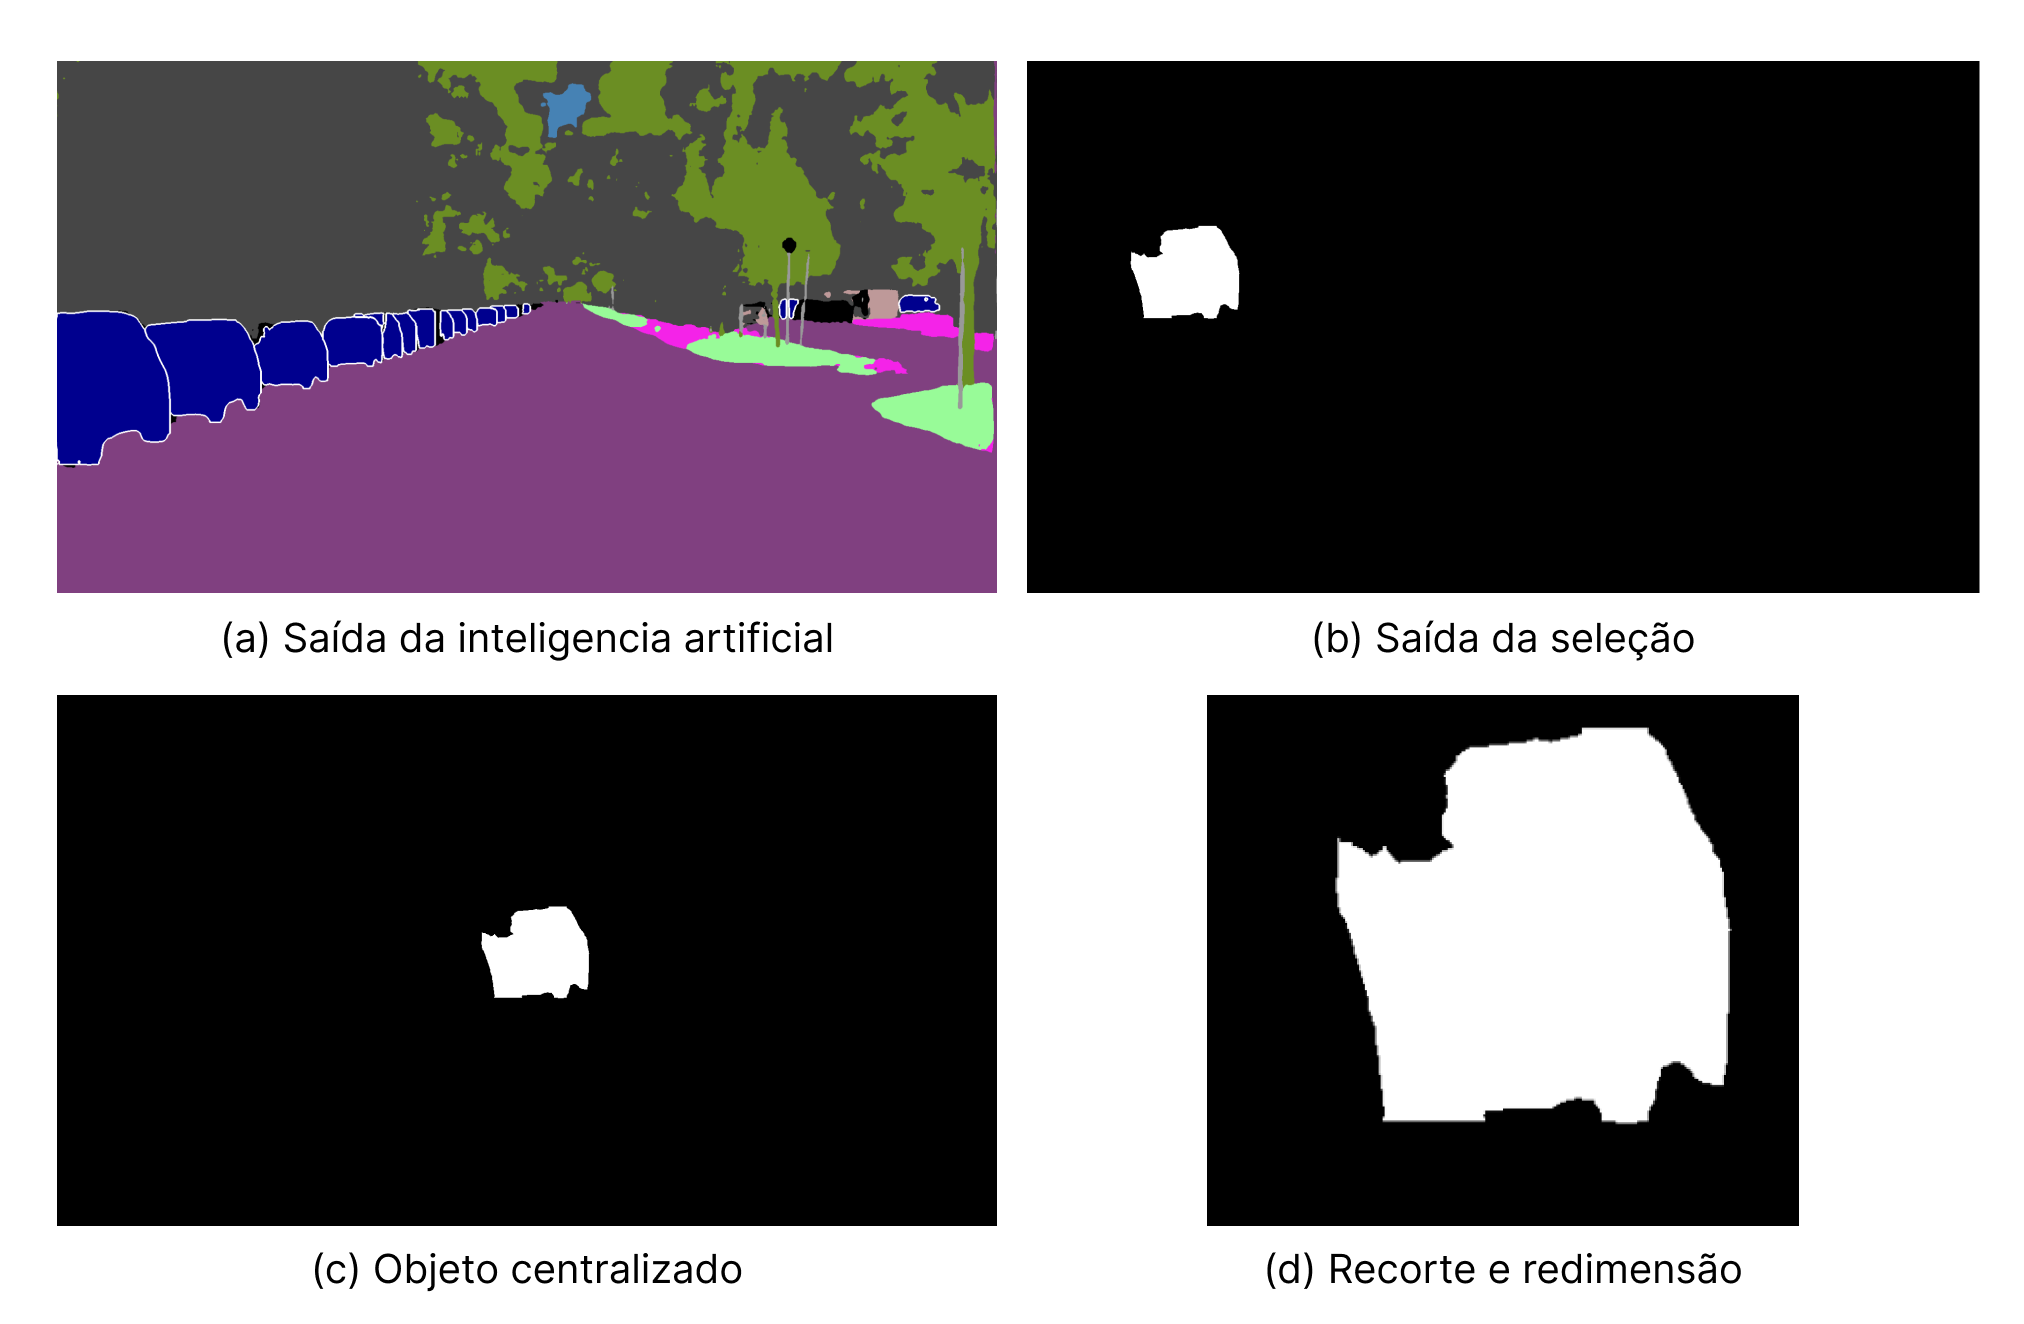
\includegraphics[width=0.6\textwidth]{figures/saidas_selecao.png}
    \legend{Fonte: \space Autoria própria}
	\label{fig:saidas_selecao}
\end{figure}